\documentclass[12pt]{article}

\usepackage{sbc-template}
\usepackage{graphicx,url}
\usepackage[brazilian]{babel}
\usepackage[utf8]{inputenc}
\usepackage[T1]{fontenc}
\usepackage{enumitem}
\usepackage{placeins}

\providecommand{\palavraschave}[1]{%
  \par\vspace{6pt}\small\noindent\textbf{\textit{Palavras-Chave---}} #1\par}

\sloppy

\title{An{\'a}lise da Rela{\c{c}}{\~a}o entre Clima e\\ Desempenho Agr{\'i}cola em Varginha/MG:\\ uma Abordagem com Pandas e Dados P{\'u}blicos (2015--2025)}

\author{
  Luigi Miranda Penachio\inst{1}, Rafael de Paiva Perim\inst{1}\\
  Eduardo Gomes Carvalho\inst{1}, Marcelo Mussel\inst{1}
}

\address{
  Universidade Federal de Ci{\^e}ncia e Inova{\c{c}}{\~a}o de Minas Gerais (UFCIMG)\\
  Campus Varginha -- Varginha/MG -- Brasil
  \email{luigimiranda2003@gmail.com, rafaelperim6@gmail.com}
  \email{eduardogomes@cefetmg.br, marcelo.mussel@gmail.com}
}

\begin{document}

\maketitle

\begin{abstract}
  This paper combines hourly meteorological observations from the Brazilian
  National Institute of Meteorology (INMET) with municipal agricultural
  statistics from the Brazilian Institute of Geography and Statistics (IBGE)
  to investigate whether climate anomalies explain annual crop performance in
  Varginha, southern Minas Gerais, a major coffee-producing region. We built a
  reproducible ETL pipeline in Python/Pandas covering 2015--2025, aggregated
  station A515 data into annual and phenological-window indicators, and joined
  them to PAM (crop yield) and PPM (cattle herd) data using the year as key.
  Correlation analysis, OLS regression and the Mann--Whitney test were applied.
  Long runs of zero precipitation incompatible with the local climatology were
  treated as sensor failures and imputed with monthly medians. Annual rainfall
  anomaly shows a weak, non-significant association with coffee yield
  ($\rho=0.27$, $p=0.42$); warmer flowering seasons tend to precede lower yields
  ($\rho=-0.42$, $p=0.23$), but the effect is not significant. No association was
  found for the cattle herd either. The results highlight the value of open-data
  integration, of careful sensor-quality control, and the need for longer series
  to support agronomic inference.
\end{abstract}

\begin{resumo}
  Este trabalho cruza observa{\c{c}}{\~o}es meteorol{\'o}gicas hor{\'a}rias do INMET com
  estat{\'i}sticas agropecu{\'a}rias municipais do IBGE para investigar se anomalias
  clim{\'a}ticas explicam o desempenho agr{\'i}cola anual em Varginha/MG, principal
  regi{\~a}o cafeeira do Sul de Minas. Construiu-se um pipeline ETL reproduz{\'i}vel em
  Python/Pandas para 2015--2025, agregando os dados da esta{\c{c}}{\~a}o A515 em
  indicadores anuais e de janelas fenol{\'o}gicas e cruzando-os com PAM (rendimento)
  e PPM (rebanho), tendo o ano como chave. Correla{\c{c}}{\~a}o, regress{\~a}o OLS e teste
  de Mann--Whitney foram aplicados. Sequ{\^e}ncias longas de chuva zero,
  incompat{\'i}veis com a climatologia local, foram tratadas como falha de sensor
  e imputadas pela mediana mensal. A anomalia anual de chuva apresenta
  associa{\c{c}}{\~a}o fraca e n{\~a}o significativa com o rendimento do caf{\'e}
  ($\rho=0,27$; $p=0,42$); flora{\c{c}}{\~o}es mais quentes antecedem menores rendimentos
  ($\rho=-0,42$; $p=0,23$), sem signific{\^a}ncia. Tamb{\'e}m n{\~a}o foi detectada
  associa{\c{c}}{\~a}o com o rebanho bovino. Destacam-se o valor da integra{\c{c}}{\~a}o de
  dados abertos, o controle de qualidade de sensores e a necessidade de s{\'e}ries
  mais longas.
\end{resumo}

\palavraschave{Clima; Cafeicultura; Pandas; INMET; IBGE; Ci{\^e}ncia de Dados}

\section{Introdu{\c{c}}{\~a}o}

A cafeicultura brasileira {\'e} sens{\'i}vel {\`a} distribui{\c{c}}{\~a}o de precipita{\c{c}}{\~a}o e
{\`a}s oscila{\c{c}}{\~o}es de temperatura, especialmente durante a flora{\c{c}}{\~a}o e a
forma{\c{c}}{\~a}o de frutos \cite{ipcc2021,aparecido2016}. No Sul de Minas Gerais, a
safra {\'e} colhida principalmente entre abril e agosto, e a flora{\c{c}}{\~a}o ocorre na
primavera do ano anterior, o que torna a escolha da janela temporal t{\~a}o
importante quanto a escolha da vari{\'a}vel clim{\'a}tica \cite{meireles2009}.

A cidade de Varginha/MG {\'e} um polo cafeeiro com s{\'e}rie meteorol{\'o}gica cont{\'i}nua
da esta{\c{c}}{\~a}o autom{\'a}tica A515 do INMET e com estat{\'i}sticas municipais anuais do
IBGE. Apesar da disponibilidade desses dados, ainda s{\~a}o escassos os estudos
reproduz{\'i}veis que integram as duas fontes com ferramentas computacionais
abertas. Este trabalho tem por objetivo responder: (i) anomalias de chuva e
temperatura explicam varia{\c{c}}{\~o}es anuais do rendimento do caf{\'e} em Varginha? (ii)
janelas fenol{\'o}gicas apresentam associa{\c{c}}{\~a}o mais forte que a m{\'e}dia anual? e
(iii) o rebanho bovino responde {\`a} precipita{\c{c}}{\~a}o com defasagem de um ano?

\section{Trabalhos Relacionados}

Victorino \cite{victorino2015} adaptou um modelo agrometeorol{\'o}gico de previs{\~a}o de
produtividade para Lavras e Varginha e encontrou maior sensibilidade ao d{\'e}ficit
h{\'i}drico entre novembro e abril. Aparecido et al.\ \cite{aparecido2016} calibraram
modelos de regress{\~a}o m{\'u}ltipla para seis regi{\~o}es produtoras de Minas Gerais, com
anteced{\^e}ncia de at{\'e} seis meses, e observaram que no Sul de Minas a produtividade
{\'e} controlada por m{\'u}ltiplos elementos meteorol{\'o}gicos. Gomes et al.\ \cite{gomes2026}
analisaram tend{\^e}ncias clim{\'a}ticas de 1984 a 2023 em duas unidades produtivas do
Sul de Minas e verificaram correla{\c{c}}{\~o}es de sinais opostos entre elas, atribu{\'i}das
{\`a}s condi{\c{c}}{\~o}es locais de microclima e uso do solo. Meireles e Japiass{\'u}
\cite{meireles2009} detalharam a fenologia do cafeeiro em Varginha e mostraram que a
aus{\^e}ncia de chuvas em setembro e outubro compromete a flora{\c{c}}{\~a}o.

Diferentemente desses trabalhos, que empregam s{\'e}ries de esta{\c{c}}{\~o}es
especializadas ou dados de cooperativas, este artigo usa exclusivamente bases
p{\'u}blicas e um pipeline de c{\'o}digo aberto, quantificando a incerteza associada a
uma amostra curta e disponibilizando o processo de junção e limpeza em \url{https://github.com/LuigiPenachio/clima-cafe-varginha-pandas}.

\section{Metodologia}

\subsection{Extra{\c{c}}{\~a}o e jun{\c{c}}{\~a}o}

Foram utilizadas tr{\^e}s bases: (1) arquivos ZIP anuais do BDMEP/INMET
\cite{inmet2026}, contendo medi{\c{c}}{\~o}es hor{\'a}rias de todas as esta{\c{c}}{\~o}es autom{\'a}ticas
de 2015 a 2025; (2) a Pesquisa Agr{\'i}cola Municipal (PAM), tabela SIDRA 5457, com o
rendimento m{\'e}dio do caf{\'e} em gr{\~a}o (produto 40139), milho e soja no munic{\'i}pio
3170701 \cite{ibgePAM2025}; e (3) a Pesquisa da Pecu{\'a}ria Municipal (PPM), tabela
3939, com o efetivo de bovinos \cite{ibgePPM2025}. A esta{\c{c}}{\~a}o A515 est{\'a} localizada
no pr{\'o}prio munic{\'i}pio (latitude $-21{,}5664^\circ$, longitude $-45{,}4042^\circ$),
portanto a chave de jun{\c{c}}{\~a}o adotada foi o \textbf{ano}, com esta{\c{c}}{\~a}o e
munic{\'i}pio como atributos fixos. As janelas fenol{\'o}gicas que envolvem a
flora{\c{c}}{\~a}o foram calculadas com o ano anterior ao da colheita.

\subsection{Limpeza e agrega{\c{c}}{\~a}o}

Os CSVs do INMET usam dois layouts: at{\'e} 2018, datas no formato
\texttt{AAAA-MM-DD}, horas \texttt{HH:MM} e valor ausente $-9999$; a partir de 2019,
datas \texttt{AAAA/MM/DD}, horas \texttt{HHMM UTC} e campos vazios. Ambos foram
normalizados. Dias com menos de seis horas v{\'a}lidas e meses com menos de 15 dias
v{\'a}lidos foram descartados. Os dados hor{\'a}rios foram agregados em totais e
m{\'e}dias mensais e anuais: precipita{\c{c}}{\~a}o acumulada, temperatura m{\'e}dia,
temperatura m{\'a}xima m{\'e}dia e contagem de dias com m{\'a}xima acima de $35^\circ$C.
A an{\'a}lise de qualidade detectou sequ{\^e}ncias de tr{\^e}s ou mais meses com
precipita{\c{c}}{\~a}o zero (mai--jul/2019, mai--jul/2022, mai--dez/2023 e
jan--mar/2024), incompat{\'i}veis com a climatologia local e indicativas de falha
do sensor. Esses 17 meses e os dois meses ausentes (ago/2016 e dez/2025) foram
imputados pela mediana mensal do per{\'i}odo, totalizando 19 meses sinalizados no
painel. Anomalias z foram calculadas por vari{\'a}vel usando o per{\'i}odo
2015--2025 como linha de base, e os rendimentos foram winsorizados nos percentis
1\% e 99\%.

\subsection{T{\'e}cnicas estat{\'i}sticas}

Foram empregadas correla{\c{c}}{\~o}es de Pearson e Spearman, regress{\~a}o linear OLS com
modelos de uma e duas vari{\'a}veis (incluindo um termo quadr{\'a}tico), teste n{\~a}o
param{\'e}trico de Mann--Whitney para comparar anos secos e chuvosos, e uma regress{\~a}o
com defasagem de um ano para o rebanho bovino, al{\'e}m de uma an{\'a}lise de sensibilidade
sem os anos com sequ{\^e}ncias imputadas. As an{\'a}lises foram implementadas com
Pandas \cite{mckinney2010}, SciPy \cite{virtanen2020} e Statsmodels
\cite{seabold2010}; as figuras usaram Matplotlib e Seaborn \cite{waskom2021}.

\section{Resultados}

A Figura~\ref{fig:mapa} localiza o munic{\'i}pio e a esta{\c{c}}{\~a}o, e a
Figura~\ref{fig:clima} mostra a climatologia mensal: dezembro {\'e} o m{\^e}s mais
chuvoso, seguido de janeiro, e julho e agosto s{\~a}o os mais secos, padr{\~a}o
compat{\'i}vel com o regime do Sul de Minas. No per{\'i}odo, a precipita{\c{c}}{\~a}o anual m{\'e}dia, ap{\'o}s imputa{\c{c}}{\~a}o, foi de
1048\,mm (728--1476\,mm) e a temperatura m{\'e}dia de $20{,}5^\circ$C. O rendimento
m{\'e}dio do caf{\'e} foi de 1567\,kg/ha, variando de 1038 a 2122\,kg/ha.

\begin{figure}[ht]
\centering
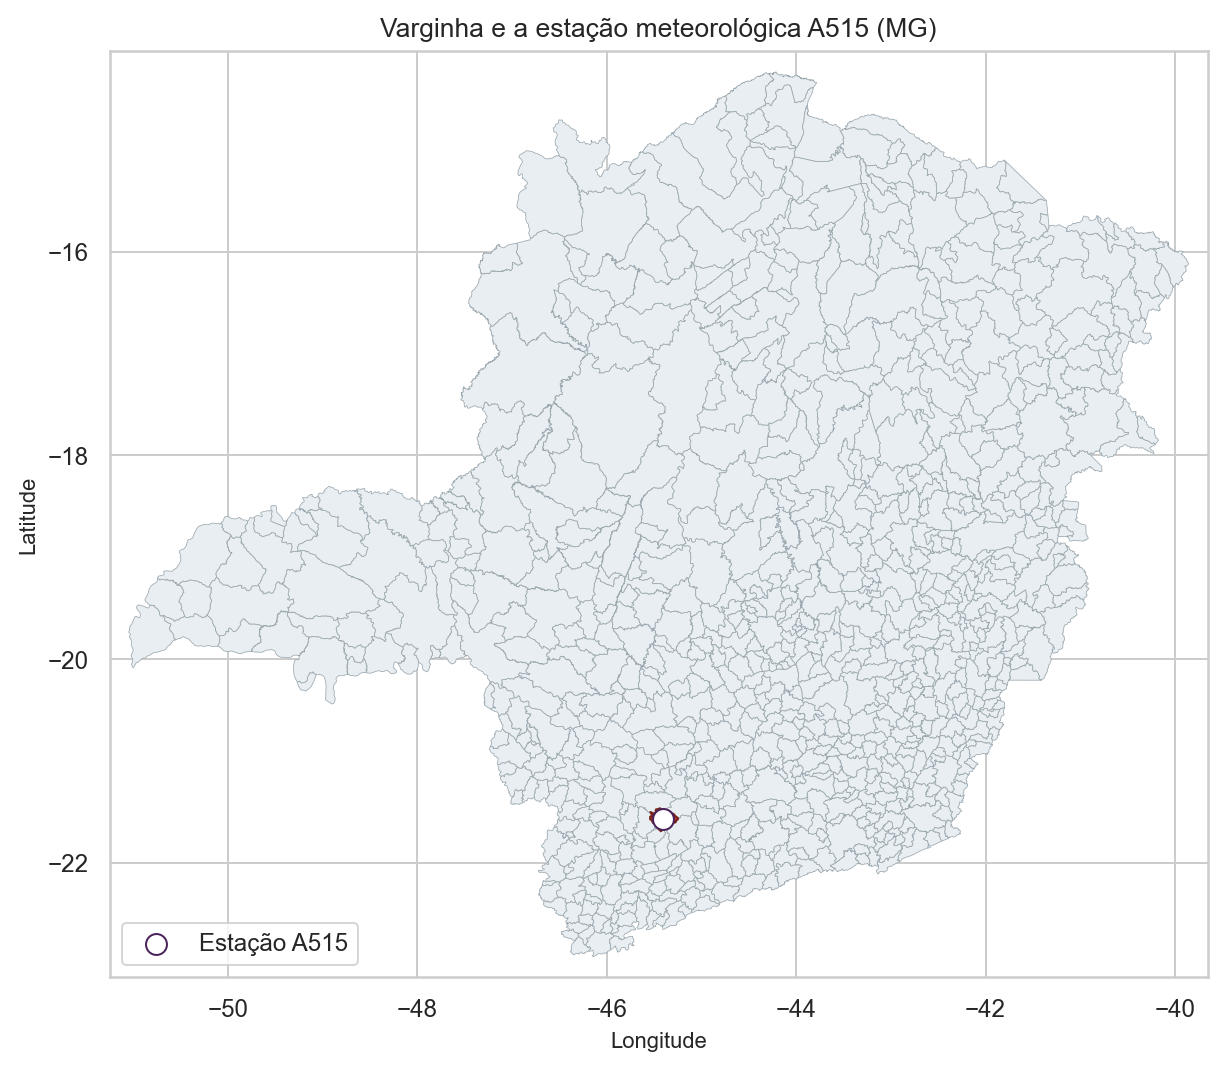
\includegraphics[width=.7\textwidth]{figuras/01_mapa_varginha.png}
\caption{Localiza{\c{c}}{\~a}o de Varginha em Minas Gerais e da esta{\c{c}}{\~a}o autom{\'a}tica A515.}
\label{fig:mapa}
\end{figure}

\begin{figure}[ht]
\centering
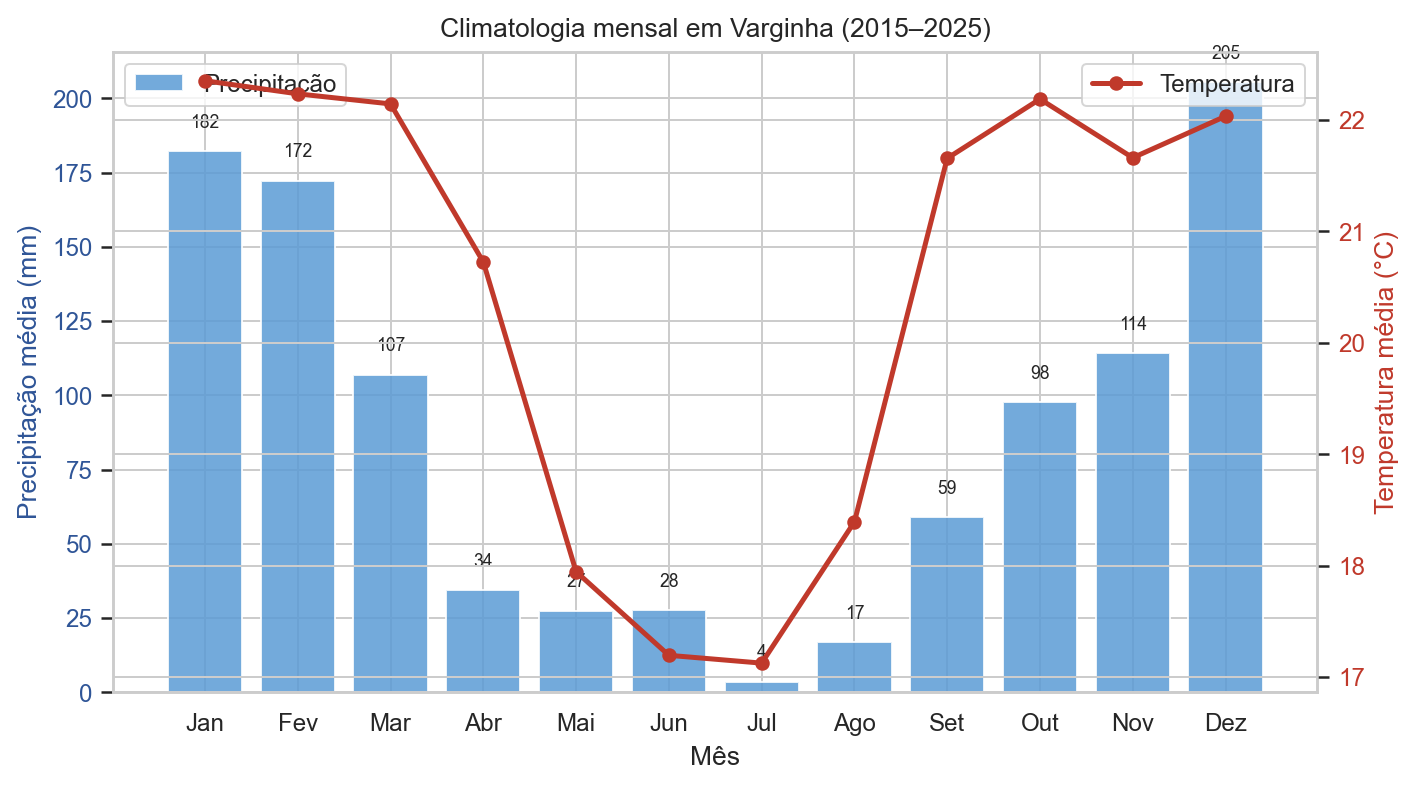
\includegraphics[width=.85\textwidth]{figuras/02_climograma.png}
\caption{Climatologia mensal de precipita{\c{c}}{\~a}o e temperatura em Varginha (2015--2025).}
\label{fig:clima}
\end{figure}

A Tabela~\ref{tab:corr} resume as correla{\c{c}}{\~o}es com o rendimento do caf{\'e}. A chuva
anual apresentou $\rho=0{,}27$ ($p=0{,}42$) e a chuva na frutifica{\c{c}}{\~a}o $\rho=0{,}41$
($p=0{,}24$); a temperatura na flora{\c{c}}{\~a}o teve $\rho=-0{,}42$ ($p=0{,}23$).
Nenhuma associa{\c{c}}{\~a}o foi significativa a 5\%. A an{\'a}lise explorat{\'o}ria por m{\^e}s
indicou rho de $0{,}45$ em janeiro e $-0{,}41$ em dezembro, tamb{\'e}m n{\~a}o significativos.

\begin{table}[ht]
\centering
\caption{Correla{\c{c}}{\~a}o de Spearman entre indicadores clim{\'a}ticos e anomalia do rendimento do caf{\'e}.}
\label{tab:corr}
\begin{tabular}{lccc}
\hline
Vari{\'a}vel & n & $\rho$ & $p$ \\
\hline
Chuva na frutifica{\c{c}}{\~a}o & 10 & 0,41 & 0,24 \\
Chuva anual & 11 & 0,27 & 0,42 \\
Chuva na colheita & 11 & 0,19 & 0,58 \\
Chuva na flora{\c{c}}{\~a}o & 10 & 0,22 & 0,53 \\
Temperatura m{\'e}dia & 11 & $-0{,}01$ & 0,99 \\
Dias quentes & 11 & $-0{,}05$ & 0,89 \\
Temperatura na flora{\c{c}}{\~a}o & 10 & $-0{,}42$ & 0,23 \\
\hline
\end{tabular}
\end{table}

Os modelos OLS n{\~a}o explicaram a varia{\c{c}}{\~a}o do caf{\'e}: o modelo com chuva anual
teve $R^2=0{,}04$ ($p=0{,}54$); com chuva na frutifica{\c{c}}{\~a}o e calor na flora{\c{c}}{\~a}o,
$R^2=0{,}21$ ($p=0{,}45$); e o modelo quadr{\'a}tico, $R^2=0{,}09$ ($p=0{,}68$). O teste de
Mann--Whitney entre anos secos e chuvosos tamb{\'e}m n{\~a}o rejeitou a hip{\'o}tese nula
($U=5{,}5$; $p=1{,}00$). A Figura~\ref{fig:scan} ilustra a rela{\c{c}}{\~a}o fracamente
positiva entre chuva anual e rendimento.

\begin{figure}[ht]
\centering
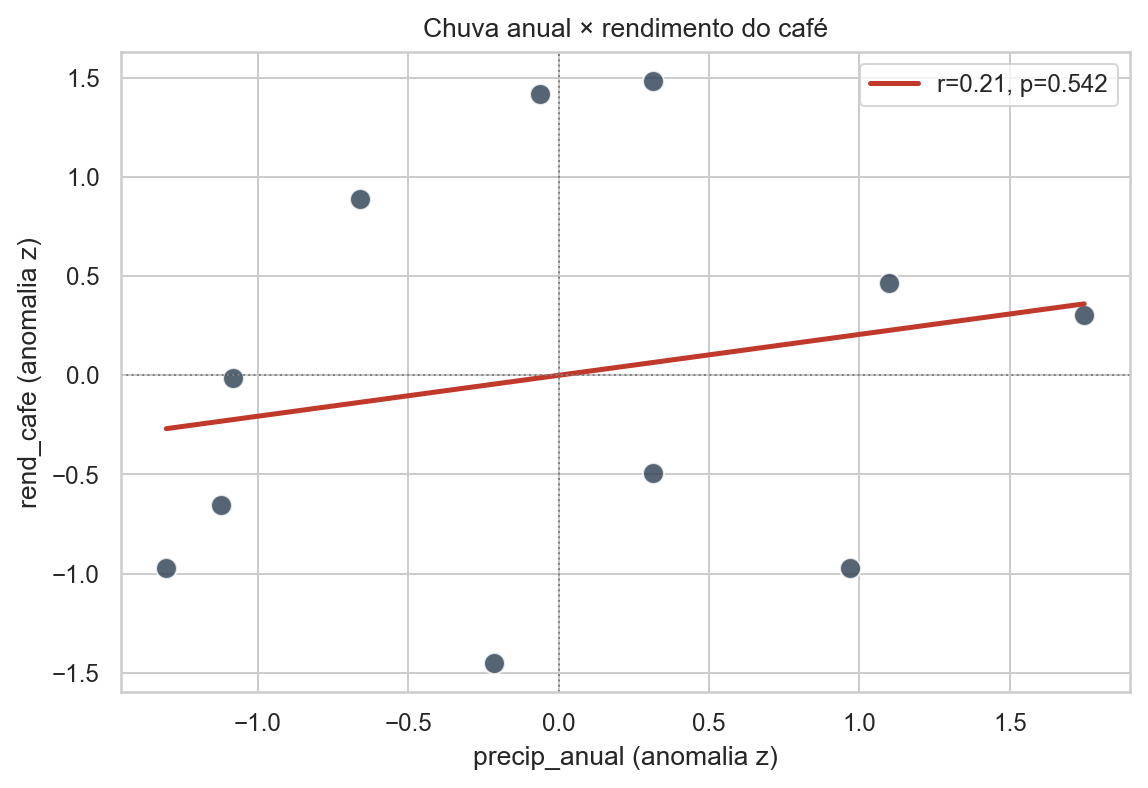
\includegraphics[width=.8\textwidth]{figuras/04_dispersao_chuva_cafe.png}
\caption{Anomalia de precipita{\c{c}}{\~a}o anual versus anomalia do rendimento do caf{\'e}.}
\label{fig:scan}
\end{figure}

A regress{\~a}o do rebanho bovino contra a anomalia de chuva do ano anterior n{\~a}o
mostrou associa{\c{c}}{\~a}o ($\beta=0{,}03$; $R^2=0{,}001$; $p=0{,}94$; $n=10$), como
ilustra a Figura~\ref{fig:rebanho}. A an{\'a}lise de sensibilidade, excluindo os anos com
sequ{\^e}ncias longas imputadas ($n=7$), manteve o resultado nulo para a chuva anual
($\rho=0{,}23$; $p=0{,}61$; $n=7$) e sugeriu uma associa{\c{c}}{\~a}o negativa entre calor na
flora{\c{c}}{\~a}o e rendimento ($\rho=-0{,}89$; $p=0{,}019$; $n=6$), interpretada com cautela
devido ao tamanho amostral e {\`a} multiplicidade de testes.

\begin{figure}[ht]
\centering
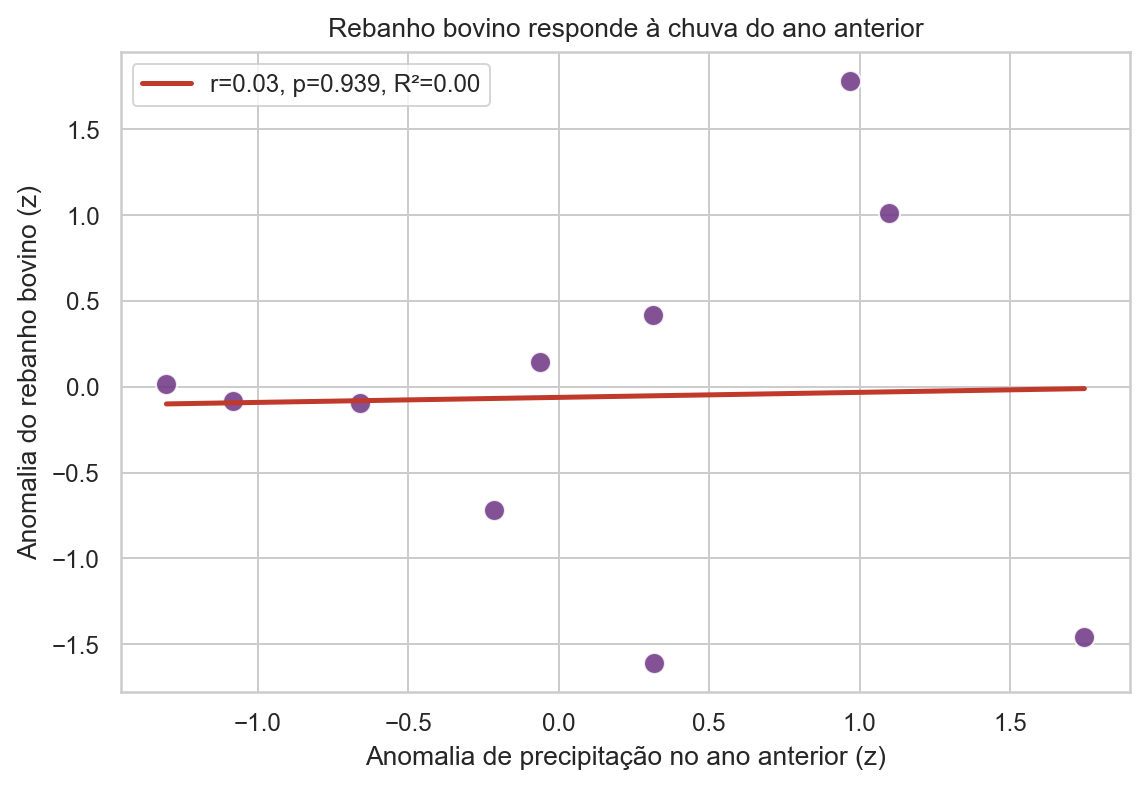
\includegraphics[width=.8\textwidth]{figuras/09_rebanho_chuva_atrasada.png}
\caption{Rebanho bovino versus anomalia de precipita{\c{c}}{\~a}o do ano anterior.}
\label{fig:rebanho}
\end{figure}

\section{Discuss{\~a}o}

Os resultados n{\~a}o confirmam a hip{\'o}tese de que a chuva anual explica o rendimento
do caf{\'e} em Varginha. A detec{\c{c}}{\~a}o e imputa{\c{c}}{\~a}o de sequ{\^e}ncias de chuva zero
foi decisiva: sem esse controle, os meses defeituosos geravam uma correla{\c{c}}{\~a}o
esp{\'u}ria com o rebanho bovino ($R^2=0{,}54$), que desapareceu ap{\'o}s a corre{\c{c}}{\~a}o.
Isso n{\~a}o contradiz a literatura: Victorino
\cite{victorino2015} e Aparecido et al.\ \cite{aparecido2016} obtiveram modelos
{\'u}teis ao usar vari{\'a}veis de d{\'e}ficit h{\'i}drico e m{\'u}ltiplas janelas mensais,
enquanto Gomes et al.\ \cite{gomes2026} encontraram correla{\c{c}}{\~o}es divergentes entre
unidades pr{\'o}ximas. A dire{\c{c}}{\~a}o negativa da temperatura na flora{\c{c}}{\~a}o e a
dire{\c{c}}{\~a}o positiva da chuva de janeiro s{\~a}o coerentes com a fenologia descrita
por Meireles e Japiass{\'u} \cite{meireles2009}, mas o tamanho amostral ($n=11$) n{\~a}o
permite infer{\^e}ncia: com 11 pontos, um coeficiente de correla{\c{c}}{\~a}o pr{\'o}ximo de
$0{,}6$ j{\'a} seria necess{\'a}rio para signific{\^a}ncia a 5\%.

A aus{\^e}ncia de associa{\c{c}}{\~a}o com o rebanho bovino tamb{\'e}m pode refletir a
tend{\^e}ncia descendente da s{\'e}rie e fatores econ{\^o}micos n{\~a}o observados. Como
limita{\c{c}}{\~o}es, citam-se: uma {\'u}nica esta{\c{c}}{\~a}o, o descompasso entre ano civil e ciclo
cafeeiro, os 19 meses imputados (oito deles em 2023), fatores de confus{\~a}o n{\~a}o
observados (pre{\c{c}}o, {\'a}rea colhida, tecnologia, pragas), o car{\'a}ter preliminar dos
dados de 2025 e a multiplicidade de testes nas janelas mensais.

\section{Conclus{\~a}o}

Este trabalho demonstrou uma integra{\c{c}}{\~a}o reproduz{\'i}vel de dados clim{\'a}ticos e
agropecu{\'a}rios p{\'u}blicos para Varginha/MG. Em 11 anos, n{\~a}o foi poss{\'i}vel detectar
efeitos significativos do clima sobre o rendimento anual do caf{\'e} ou sobre o
rebanho bovino. Como contribui{\c{c}}{\~a}o, o c{\'o}digo aberto documenta o tratamento dos
dois layouts do INMET, a detec{\c{c}}{\~a}o de falhas de sensor, a jun{\c{c}}{\~a}o via API SIDRA
e as janelas fenol{\'o}gicas. Trabalhos futuros devem ampliar a s{\'e}rie, incluir
esta{\c{c}}{\~o}es vizinhas e balan{\c{c}}o h{\'i}drico, e avaliar modelos com efeitos de
bienalidade da safra.

\bibliographystyle{sbc}
\bibliography{artigo_bib}

\end{document}
